\chapter{Architecture}%
\label{chap:architecture}
The architecture for the application is composed by two main components: the Flutter application that represents the client-side and a server, hosted on Google Firebase, that represents the server-side.

In the diagram below the main components, that are described later,  and their interaction are shown.

\begin{figure}[htpb]
	\centering
	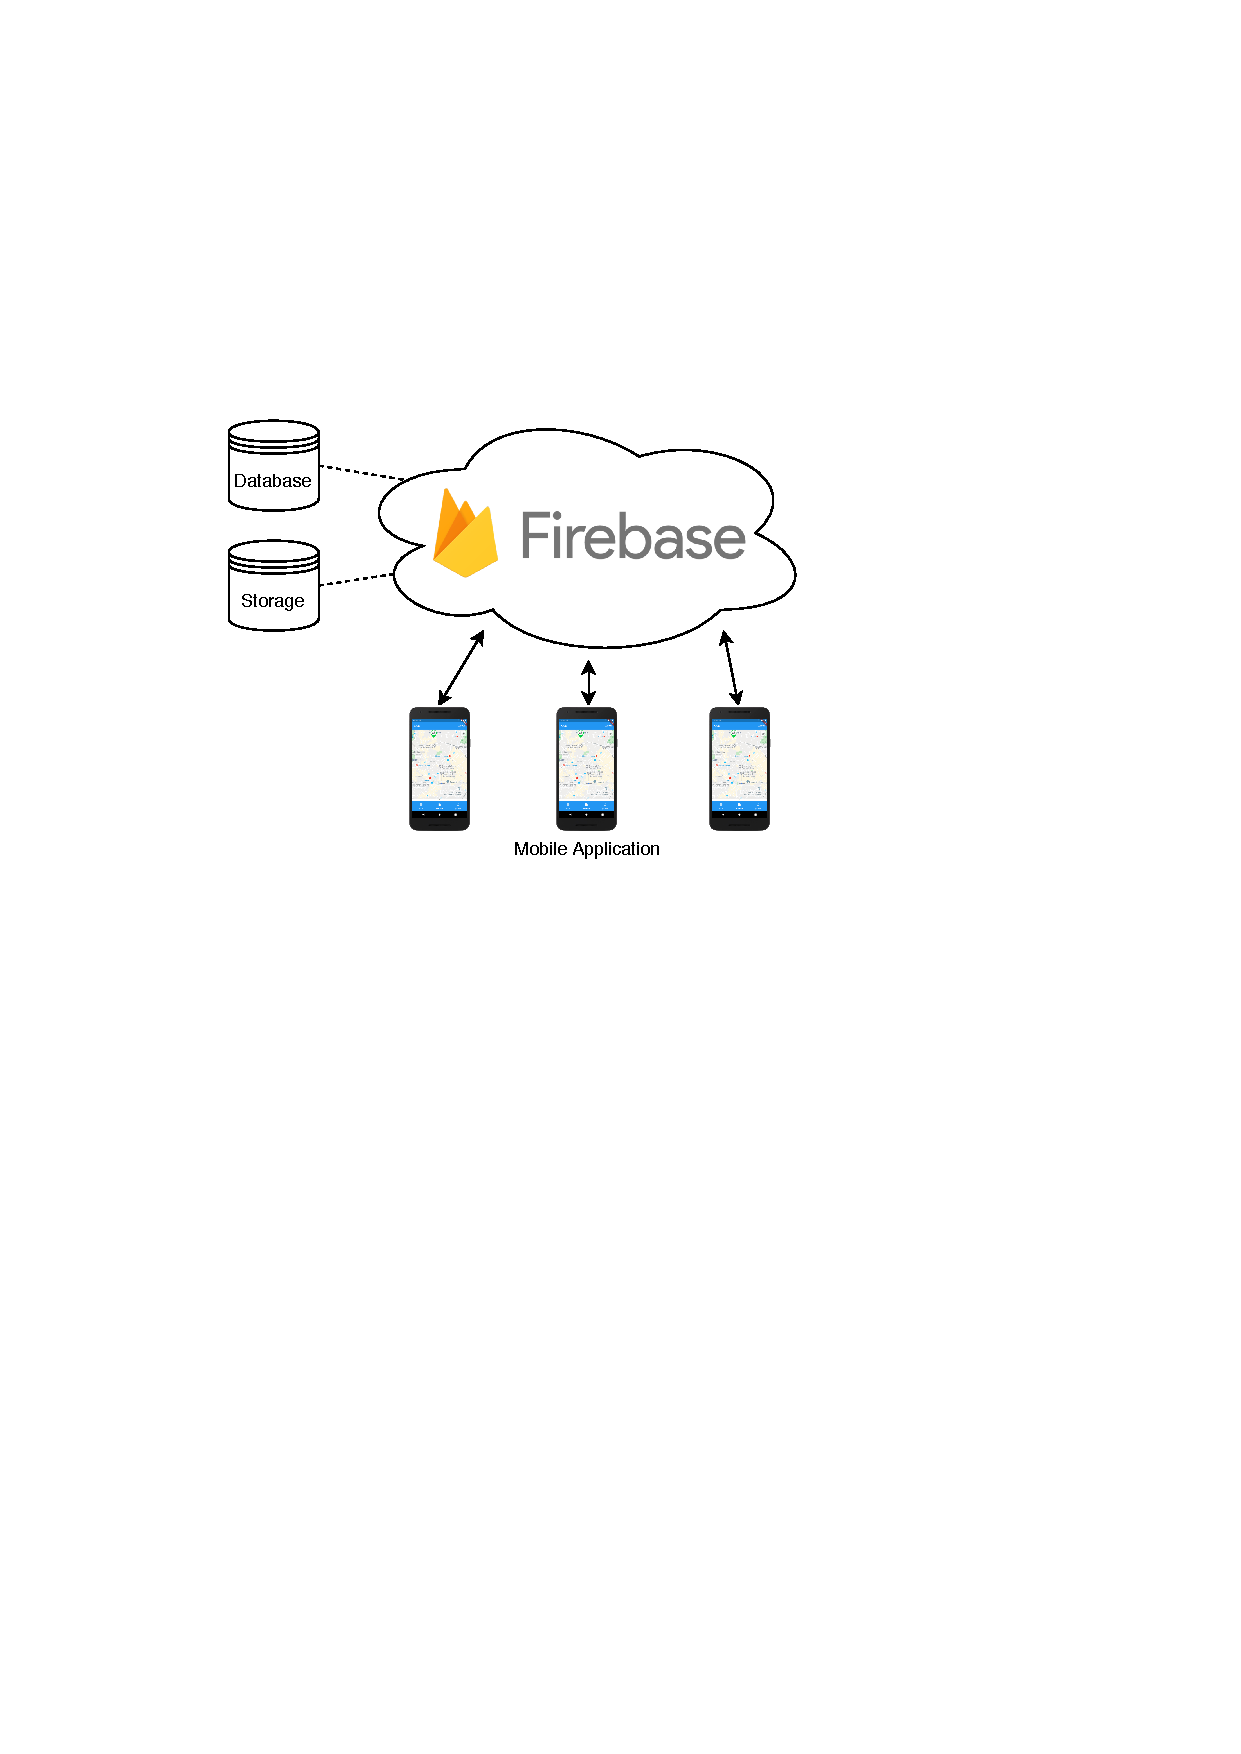
\includegraphics[width=0.9\linewidth]{Pics/architecture2.pdf}
	\caption{Basic architecture of the application.}%
	\label{fig:Pics/architecture}
\end{figure}

\section{Client-side application}
This part is represented by the Flutter application and is most of the written code. The functional components and the graphical ones are not strictly separated, everything is built with the official Widgets provided by Flutter. 

Widgets are elements of interaction in the graphical interface, they help to build UI, from basic to more complex one just combining them. 

In the client-side there are also all the functionalities to interact with the Database and Google Maps, to handle notifications and collect statistics. 
\subsection{Code package}

\begin{figure}[htpb]
	\centering
	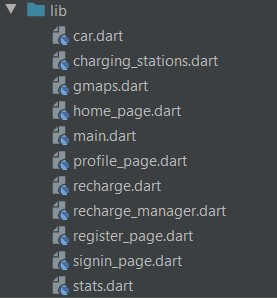
\includegraphics[width=0.4\linewidth]{Pics/code_package.jpg}
	\caption{The lib package.}%
	\label{fig:Pics/code_package}
\end{figure}

The figure above shows the lib package, where all the dart class are collected, basically each one represent a different page in the mobile application and it is the real core of the entire implementation.

The following list briefly describes the main classes: 
\begin{itemize}
	\item \textbf{main}: it is the entry point of the application that leads directly to the home page if the user is already logged in
	\item \textbf{signin\_page and register\_page}: they handle the authentication process(log in and registration)
	\item \textbf{home\_page}: it is the core of the application and where the user will spend most of the time; it is divided in three tab; statistics, maps and profile
	\item \textbf{stats}: it shows and collect all the recharges of the user, showing interesting statistics about them
	\item \textbf{gmaps}: it shows the map with the charging stations, handling navigation and ordering of the stations
	\item \textbf{profile\_page}: it shows the settings and information about the user, who can modify them here
	\item \textbf{recharge\_manager}: it handles the recharging process calculating time and cost of it and the notification system when a recharge is finished
	\item \textbf{car, charging\_stations, recharge}: they are Java-like classes that define the respective object
\end{itemize}

\section{Server-side application}
The server-side of the application is entirely hosted on Google Firebase and it is represented by Database and Storage, both of this components are fully integrated on Firebase and can be accessed and modified through the built-in console. 
This server aplication has many advantages: it offers a lot of services such as authentication, hosting and analytic, so it would be easy to add one of them in the future; as Flutter it is developed by Google so the APIs to made them work together are reliable; it is easy scalable starting from a free plan and then upgrading it. 